% !TeX program = xelatex
% CENT — Chinese handwriting LINE generation with continuity by construction
% MANUSCRIPT STATUS: method + feasibility analysis + frozen protocol.
% No comparative empirical results are reported, because none exist.
% Measured numbers come from analysis/lexicon_stats.py; metric definitions from
% benchmark/connectivity.py; every empirical claim is either computed here or cited.
% Target: CVPR (IEEE two-column; the CVPR author kit must replace IEEEtran).
\documentclass[conference]{IEEEtran}
\usepackage{iftex}
\ifXeTeX
  \usepackage{fontspec}
  \IfFontExistsTF{Times New Roman}{\setmainfont{Times New Roman}}{}
  \usepackage{xeCJK}
  \IfFontExistsTF{Microsoft YaHei}{\setCJKmainfont{Microsoft YaHei}}{}
\fi
\usepackage{amsmath,amssymb}
\usepackage{graphicx}
\usepackage{booktabs}
\usepackage{array}
\usepackage{tikz}
\usetikzlibrary{arrows.meta,positioning,fit,backgrounds,calc}
\usepackage{url}
\usepackage[hidelinks]{hyperref}
\usepackage{balance}

\begin{document}

\title{CENT: Chinese Handwriting Line Generation\\with Continuity by Construction}

\author{\IEEEauthorblockN{Anonymous CVPR submission}
\IEEEauthorblockN{Paper ID ****}
\IEEEauthorblockA{Confidential review copy. Do not distribute.}}

\maketitle

\begin{abstract}
Chinese handwritten line generation is largely solved at the glyph and unsolved at the seam.
Layout-decoupled models place glyphs in predicted boxes, and their own reports concede that
they cannot express a connection between characters; sequence models can express one, but only
as an implicit by-product of a pen-state label, which encourages continuity without guaranteeing
it. We make continuity a property of the representation. A line is a stroke sequence in which
every stroke is a \emph{relative} offset from the current pen position, so the path is a running
sum that cannot jump, and every character boundary carries an explicit \emph{contract}: a join
decision together with the exit and entry anchors and a bridge, from which the first stroke of
the next character is forced to begin. A joined boundary therefore has a start offset of exactly
zero, not small. Four modules carry four disjoint responsibilities --- content, writer style,
layout, and the boundary --- which we state as a responsibility matrix so that each claim in this
paper is attributable to the module that makes it, and we separate three senses of coherence
(pen-path continuity, inter-character connection, line-level rhythm) that are routinely
conflated into a single join rate. We also report a development finding that constrains the
whole problem: an offline scan and an online trajectory of the same text are different writing
sessions, so a scan cannot serve as a pixel target for a trajectory, and paired corpora support
style supervision but not geometric supervision. This manuscript reports the method, a staged
falsification protocol and development evidence; it reports no comparison against baselines.
\end{abstract}

\begin{IEEEkeywords}
handwriting generation, Chinese script, text lines, cursive connectivity, structured
representations, evaluation methodology
\end{IEEEkeywords}

\section{Introduction}

Synthetic Chinese handwriting has three credible uses: augmenting training data for
handwritten text recognition, producing a personal font from a handful of samples, and
teaching stroke order. All three are line-level tasks in practice --- recognition consumes
lines, and a font that cannot set a line is not a font.

The glyph half of this problem is in good shape. Diffusion and transformer models generate
convincing Chinese characters in a target style from a few references
\cite{sdt,metascript,hisac,diffwriter,dp_font,scfont,stroke2font,lvgh}. A line generator that
inherited only that ability would already produce recognisable text. The gap is at the seam
between characters, and it is not a rendering artefact: it is the difference between a row
of written glyphs and a line someone wrote quickly.

Two families handle that seam badly in opposite ways. \emph{Layout-decoupled} methods predict
a box per character and fill it \cite{layout_glyph,hct_gan,yao2025}. By construction no stroke
may cross a box boundary, so a join cannot occur; the authors of the closest such system
concede that independent per-character generation ``encounters difficulties in mimicking
styles with extensive cursive connections between characters'' \cite{layout_glyph}. It is
worth being precise about this: it is not a training deficiency but a representational one.
CENT keeps the layout \emph{plan} while dropping both of its usual consequences. Our anchors
$a_i=(x_i,y_i,w_i,h_i,\Delta x_i)$ are soft: they enter the decoder as a neighbourhood
conditioning signal $(a_{i-1},a_i,a_{i+1})$ added to the transcript memory, strokes are never
clipped to them, and the boundary contract of \S\ref{sec:method} is unchanged. The anchor is
therefore a plan the pen may exceed, not a cell it must fill; the independence that forbids a
join is not inherited, because a connector is generated between two anchors rather than inside
either.
\emph{Sequence} methods instead emit one long pen trajectory \cite{graves2013,diffink,sdt},
and here joins do appear, but as an implicit consequence of a pen-down label. That is a
weaker guarantee than it looks: the label says the pen did not lift, and says nothing about
the direction it was travelling, so two independently predicted segments can meet at an
angle at exactly the moment the model claims continuity.

Explicit connection models existed long before either family, in the handwriting-synthesis
literature of the 2000s \cite{lin2007,wang2005,chen2015}, which separated a character model
from a \emph{connection} model: a per-pair probability of joining, plus a ligature stroke
whose endpoints were tied to the tails and heads of its neighbours, fused by minimising an
energy that included a direction-alignment term. That formulation is the right one, and it
was built for writer-specific template systems on Latin script, before content-generalising
generative models existed. Recently the boundary has returned as an explicit object of study:
BoundInk \cite{boundink} treats inter-character boundaries as generation units, supervises a
pen state that means ``end of character with the pen still down'', and defines a boundary-aware
metric suite. Its own results make our point and also set our problem: under the Chinese
protocol it compares on, the suite collapses --- only spacing is defined, because the
evaluation set contains no cursive-positive boundaries at all. In Chinese, connectivity is
not merely unmodelled; it is currently unmeasurable.

\subsection{The proposal}
CENT is a line model that treats the connector as a first-class object with a geometry, and
then arranges for continuity to be a property of that geometry rather than a hope.

\begin{enumerate}
\item \textbf{A line is a relative stroke sequence.} Each stroke is an offset from the current
pen position, so the pen path is a running sum and cannot jump. Character identity enters
through the transcript by cross-attention, not through a fixed per-character stroke topology:
cursive execution merges strokes, and a lexicon-fixed count cannot express that.
\item \textbf{Continuity by construction.} Every boundary carries a contract --- a join decision
plus exit and entry anchors --- from which the first stroke of the next character is forced to
begin. A joined boundary therefore starts at offset exactly zero, and no classifier can trade
the guarantee away.
\item \textbf{Joining is a decision, conditioned on the writer.} A per-boundary Bernoulli
variable the model predicts and can override, conditioned on the writer's own join rate and on
an empirical per-pair prior measured from the reference statistics.
\item \textbf{One latent, two decodes.} Ordered curve evaluation gives a trajectory with exact
pen lifts; rasterisation gives the line image. Because the join decision lives in the shared
geometry, the two outputs cannot disagree about it.
\end{enumerate}

\subsection{Contributions}
\begin{itemize}
\item \textbf{Continuity as a guarantee of the parameterisation.} Each stroke is an offset from
the current pen position and each boundary carries a contract that fixes the offset of the next
character's first stroke. A joined boundary has a start offset of exactly zero, so the
discontinuity is not small but absent, and what remains learned --- and therefore falsifiable
--- is whether a writer joins at all and how sharply the pen turns (Section~\ref{sec:method}).
\item \textbf{A responsibility matrix for line generation.} Content, writer style, layout and
the boundary are assigned to disjoint modules (M1--M8) rather than to one latent sequence, so
every reported number names the module that produced it. We additionally separate three senses
of coherence that prior work reduces to a single join statistic.
\item \textbf{A negative result that bounds the data.} On CASIA's paired lines we measure that
the scan and the trajectory of the same text are different writing sessions: after removing any
frame offset, the IoU between a rendered trajectory and its paired scan is $0.008$--$0.013$.
Paired corpora therefore supervise \emph{style}, not geometry --- a constraint that any method
training on paired offline/online data must respect.
\item \textbf{Connectivity metrics that stay defined in Chinese.} The boundary-aware suite of
\cite{boundink} degenerates without word spaces; we adopt its join F1, join-rate error and gap
similarity, state which definitions are ours, and add a continuity error that scores direction
at the join.
\end{itemize}

\subsection{Status of this manuscript}
We report the method, the module decomposition, a staged falsification protocol and a negative
development result. \emph{We report no comparison against baselines.} During development we
trained ten configurations of an earlier formulation on the CASIA line corpora and none
produced a legible line, including an overfit test on a single line; those runs are summarised
in the supplement because they motivate the revision rather than support it. The architecture
described here has been implemented and syntax-checked but not yet trained, so no number in
this paper is a measurement of the present system except the corpus statistics and the
paired-session IoU, both of which are measurements of data.
\section{Related Work}

\subsection{Offline text-line generation}
DiffBrush \cite{diffbrush} learns line-level style with row- and column-wise content
decoupling and enforces global coherence with line and word discriminators. TGC-Diff
\cite{tgc_diff} cascades a spatial-style model and a glyph-style model through a template.
InkSpire \cite{inkspire} unifies style, content and noise in one latent and supports masked
infilling. All three synthesise the line as an image, so any connectivity is emergent in
pixels: not switchable, not inspectable before rendering, and --- until Section~\ref{sec:protocol}
--- not scorable.

\subsection{Online line generation and the boundary}
DiffInk \cite{diffink} generates a whole line as a pen trajectory with a latent diffusion
transformer, and argues that decoupled pipelines ``mechanically stitch bounding boxes'' while
direct generation yields more natural connections; it also observes that stitching artefacts
are detectable by a style classifier. OLHWG \cite{layout_glyph} is the explicit decoupled
route: an LSTM places character boxes and a diffusion synthesizer paints each glyph into its
box, with the connectivity limitation its own report describes. BoundInk \cite{boundink}
returns the boundary to the centre of the problem, modelling predecessor--current transitions
with a sliding-window decoder and supervising a four-way pen state whose cursive class means
``end of character, pen still down'', plus a boundary-aware metric suite. Our debt to it is
direct: it establishes that boundary behaviour is a legitimate object of study and that
long-range sequence modelling captures it only implicitly.

\subsection{Connection models before deep generation}
The classical synthesis literature separated the character from the connection. Lin and Wan
\cite{lin2007} sampled, for each adjacent pair, whether to connect them --- decoupling a
writer-independent pair prior from a writer-level cursiveness scalar --- and fitted the
ligature with a polynomial. Wang \emph{et al.} \cite{wang2005} built a tri-unit model in which
the head and tail of each character and the concatenation stroke between them are separate
generative models, fused by minimising a concatenation energy that includes a
direction-alignment term and a gap term. Chen \emph{et al.} \cite{chen2015} extended the same
idea to conjoined paragraphs with trajectory optimisation over a cursive probability. These
systems are the origin of the formulation we instantiate: a join decision plus a connector
stroke plus an explicit smoothness objective. They were writer-specific template models on
Latin script; what changed is that a generative model can now generalise the glyph content,
which makes the connection the remaining degree of freedom.

\subsection{Chinese line generation with connecting strokes}
UniCalli \cite{unicalli} generates Chinese calligraphy at column level and reports ligature
continuity as an explicit quality axis, producing connecting strokes appropriate to adjacent
characters. HCT-GAN \cite{hct_gan} regulated components to build arbitrary-length Chinese
lines, and a recent style-control system \cite{yao2025} pairs a character generator with a
layout stage. These establish that Chinese inter-character strokes are generatable, and
delimit our difference: calligraphic columns are a different hand from everyday handwriting,
and the layout-stage designs inherit the box boundary. Chinese character-level systems
\cite{metascript,sdt,rcgan,hisac,diffwriter} and font-oriented models
\cite{dp_font,scfont,stroke2font,lvgh,calligan,cffont,dgfont,difffont,fontdiffuser,lffont}
supply the glyph quality we build on; word-level Latin systems
\cite{ganwriting,hwt,vatr,vatr_pp,diffusionpen,one_dm,wordstylist,emuru,scriptvit,dsd,hi_gan}
are context for what a line model must add, and are Latin-only, so they cannot enter a
Chinese comparison as rows.

\subsection{What is actually new here}
Connectivity is modelled; it is modelled as a label or as box placement; and in Chinese it is
unmeasured. Our claims are therefore deliberately narrow. \emph{First}, continuity is a
consequence of the connector's parameterisation rather than of a classifier, which is a
mechanism difference with an observable signature (direction error at the join) that the
existing suite does not measure. \emph{Second}, connectivity is conditioned on the writer's
own join statistics from reference lines, so the join rate is a target statistic rather than
an emergent property. \emph{Third}, we make connectivity measurable for image-only systems,
which no prior work does, and we validate that proxy instead of asserting it.

\section{Method}\label{sec:method}

\subsection{Problem statement}
Given a string $C=(c_1,\dots,c_N)$ and $k$ reference lines $S_w$ in a target hand, CENT emits a
stroke sequence
\begin{equation}
G=(s_1,\dots,s_M),\qquad s_k=(\Delta_k,\,p_k),\; a_k\in\{1,\dots,N\},
\end{equation}
where $\Delta_k\in\mathbb{R}^{8}$ is a \emph{relative} payload: the offset from the current pen
position to the stroke's start, followed by three cubic B\'ezier control offsets relative to
that start; $p_k\in\{0,1\}$ is the pen state; and $a_k$ is the character the stroke belongs to.
Because every payload is relative, the trajectory is the running sum of the starts, and a jump
is not representable: continuity of the pen path is a property of the parameterisation rather
than a penalty in the loss.

\subsection{Three senses of coherence}
A line can be coherent in three independent ways. Conflating them is what lets a model satisfy
one while failing the others, so we separate them and name the module responsible for each.

\begin{table}[t]
\centering\small
\begin{tabular}{@{}p{0.36\columnwidth}p{0.34\columnwidth}p{0.20\columnwidth}@{}}
\toprule
sense of coherence & mechanism & module \\
\midrule
pen-path continuity & relative payload $+$ pen state & M5 (structural) \\
inter-character connection & explicit join decision $+$ boundary contract & M4 (planned) \\
line-level rhythm & autoregressive layout conditioned on style & M3 (learned) \\
\bottomrule
\end{tabular}
\caption{Three senses of coherence, kept separate. A single join-rate number conflates them;
measured on sampled output it is satisfiable by collapsing all strokes into a band.}
\label{tab:coherence}
\end{table}

\subsection{Modules and their responsibilities}
\begin{table}[t]
\centering\small
\begin{tabular}{@{}llp{0.42\columnwidth}@{}}
\toprule
module & handles & explicitly does not \\
\midrule
M1 transcript encoder & content: what to write & style, layout, boundary \\
M2 style encoder & writer identity: who writes & content, layout \\
M3$'$ soft anchors & where characters sit: $a_i$ plus its neighbourhood & stroke shapes, joins \\
M4 join planner & \textbf{whether and where two characters connect} & glyph interiors \\
M5 stroke decoder & stroke geometry, order, \textbf{pen-path continuity} & which character \\
M6 Gaussian memory mask & which character a stroke belongs to & content, style \\
M7 writer head & writer identification (auxiliary supervision) & generation \\
M8 boundary refinement & C$^1$ smoothness at joins (inference only) & the join decision \\
\bottomrule
\end{tabular}
\caption{Responsibility matrix. Disjointness is the point: each reported metric names one module.}
\label{tab:modules}
\end{table}

\subsection{The boundary contract}
For boundary $i$, between characters $c_i$ and $c_{i+1}$,
\begin{align}
\zeta_i &= \sigma\big(\mathrm{M4}(H_i,H_{i+1},B_i,B_{i+1},P(c_i,c_{i+1}),z_\kappa)\big),\\
\mathrm{gap}_i &= \mathrm{entry}_i-\mathrm{exit}_i,\\
\Delta_{\text{first stroke of }c_{i+1}} &= \mathrm{exit}_i+\mathrm{gap}_i\,(1-\zeta_i),
\end{align}
where $H$ are transcript states, $B$ layout boxes, $P$ the empirical per-pair join prior of
\cite{lin2007} restored as an input, and $z_\kappa$ the connector style code. When $\zeta_i=1$
the start offset is exactly zero. Continuity is thus a coordinate the decoder must hit, not a
label it must infer: this replaces the auxiliary join classifier of our earlier diffusion
formulation, whose F1 of $0.153$ fell below the always-join baseline of $0.339$.

\subsection{Alignment}
The transcript and the stroke sequence differ in length by an unknown factor, so M5 attends to
the transcript through a Gaussian memory mask $\mathrm{M}_{t,j}=-((j-\mu_t)^2/2\sigma^2)$ centred
on the character a stroke belongs to, with $\sigma=1$. \cite{trink} reports a character error
rate of $8.5$ with this mask against $14.9$ for a uniform local window, $14.1$ for exponential
decay and $70.1$ without any mask; the uniform variant is what an earlier revision of CENT used.

\subsection{Objectives}
\begin{align}
\mathcal{L} = {}& \underbrace{-\log p_\theta(\Delta_k\mid s_{<k},C,S_w)}_{\text{stroke (M5)}}
+ \lambda_1\underbrace{\mathrm{BCE}(\hat p_k,p_k)}_{\text{pen state}}
+ \lambda_2\underbrace{\mathrm{BCE}(\widehat{\mathrm{stop}}, \mathrm{stop})}_{\text{character end}}\notag\\
&+ \lambda_3\underbrace{\|a-\hat a\|_1}_{\text{anchors (M3$'$)}}
+ \lambda_c\underbrace{\|\Delta^2\hat a\|_1}_{\text{continuity}}
+ \lambda_4\underbrace{\mathrm{BCE}(\hat\zeta,\zeta)}_{\text{join (M4)}}
+ \lambda_5\underbrace{\|\mathrm{gap}-\widehat{\mathrm{gap}}\|_1}_{\text{anchors (M4)}}
+ \lambda_6\underbrace{\mathrm{CE}(w,\hat w)}_{\text{writer (M7)}} .
\end{align}
No pretrained generator is used: the target is a sequence of control points, twenty times
smaller than the line it renders, so a pretrained text-to-image network has no tensor to load.
The only pretrained networks are frozen evaluation extractors and contribute no parameters.

\subsection{Inference}
M3$'$ plans soft anchors, M4 decides the boundaries and their anchors, M5 decodes strokes
autoregressively with the contract applied to the first stroke of each character, and M8 rotates
the incoming control point at a joined boundary when the tangent mismatch exceeds $35^\circ$,
moving no endpoint. Layout, join decision and stroke decoding are separately interpretable and
separately ablatable.

\begin{figure*}[t]
\centering
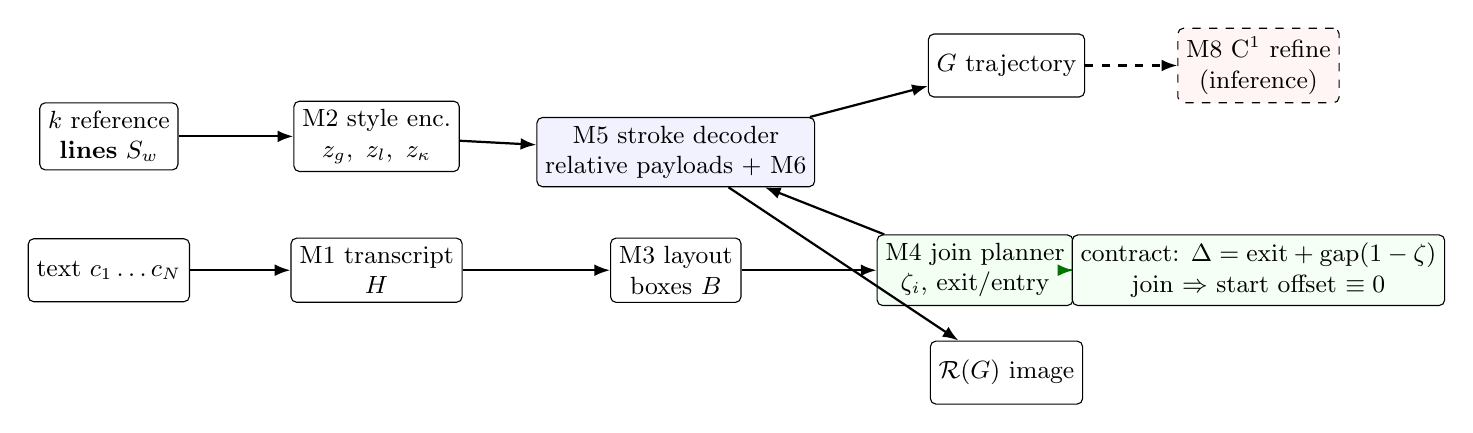
\begin{tikzpicture}[
  box/.style={draw, rounded corners=2pt, align=center, font=\small, inner sep=3pt, minimum height=8mm},
  arr/.style={-{Latex[length=2mm]}, thick},
  lab/.style={font=\scriptsize\itshape, text=black!65}]
\node[box] (ref) at (0,0) {$k$ reference\\ \textbf{lines} $S_w$};
\node[box] (sty) at (3.4,0) {M2 style enc.\\ $z_g,\ z_l,\ z_\kappa$};
\node[box] (txt) at (0,-1.7) {text $c_1\dots c_N$};
\node[box] (enc) at (3.4,-1.7) {M1 transcript\\ $H$};
\node[box] (lay) at (7.2,-1.7) {M3 layout\\ boxes $B$};
\node[box, fill=green!5] (join) at (11.0,-1.7) {M4 join planner\\ $\zeta_i$, exit/entry};
\node[box, fill=blue!5] (den) at (7.2,-0.2) {M5 stroke decoder\\ relative payloads $+$ M6};
\node[box] (traj) at (11.4,0.9) {$G$ trajectory};
\node[box] (img) at (11.4,-3.0) {$\mathcal{R}(G)$ image};
\node[box, fill=red!4, dashed] (ref8) at (14.6,0.9) {M8 C$^1$ refine\\(inference)};
\node[box, fill=green!4] (anchor) at (14.6,-1.7) {contract: $\Delta=\mathrm{exit}+\mathrm{gap}(1-\zeta)$\\ join $\Rightarrow$ start offset $\equiv 0$};
\draw[arr] (ref) -- (sty);
\draw[arr] (txt) -- (enc);
\draw[arr] (enc) -- (lay);
\draw[arr] (lay) -- (join);
\draw[arr] (sty) -- (den);
\draw[arr] (join) -- (den);
\draw[arr] (den) -- (traj);
\draw[arr] (den) -- (img);
\draw[arr, dashed] (traj) -- (ref8);
\draw[arr, green!45!black] (anchor) -- (join);
\end{tikzpicture}
\caption{CENT. Content, style, layout and the boundary are separate modules (Table~\ref{tab:modules}).
Every stroke is a relative offset, so the pen path cannot jump; M4 fixes the first offset of each
character through the boundary contract, so a joined boundary has zero start offset by
construction. The same $G$ decodes to a trajectory and, through the analytic rasteriser, to a line
image, so the two modalities cannot disagree about a join.}
\label{fig:pipeline}
\end{figure*}

\section{Is the intra-character constraint definable?}
\label{sec:analysis}
\emph{This section analyses the lexicon-fixed stroke constraint of an earlier revision. The constraint proved definable, and the analysis is what led us to abandon it: a fixed per-character stroke count cannot express cursive merging, so the present model predicts stroke sequences directly. We retain the measurement because it bounds how far a topology-first design can be pushed.}

A hard topology constraint is only defensible if the topology is known for the characters a
line may contain. We measured this on the public stroke-order lexicon \cite{hanzi} (9{,}574
characters; Arphic Public License), intersected with the GB2312 code charts;
Table~\ref{tab:lexicon} reports the result, and the script is released with the paper.

\begin{table}[t]
\centering
\caption{Topology availability and glyph complexity over the target inventory, computed from
the public stroke-order lexicon \cite{hanzi}. ``p99'' is the 99th percentile stroke count;
``$>$20'' is the fraction with more than 20 strokes.}
\label{tab:lexicon}
\small
\begin{tabular}{@{}lrrrrrr@{}}
\toprule
Inventory & \#chars & covered & mean & p99 & max & $>$20 \\
\midrule
GB2312 level-1 & 3{,}755 & 3{,}755 & 9.77 & 19 & 24 & 0.37\% \\
GB2312 level-2 & 3{,}008 & 3{,}008 & 11.69 & 22 & 30 & 1.80\% \\
GB2312 union   & 6{,}763 & 6{,}763 & 10.62 & 20 & 30 & 1.01\% \\
\bottomrule
\end{tabular}
\end{table}

Three consequences follow. First, the constraint is \emph{total} on the target inventory.
Second, the per-character target is \emph{small}: a median of 10 strokes means the character
tokens are tens of control points, and a line's length is dominated by connectors and layout
--- which is where a line model's capacity should sit. Third, complexity is
\emph{concentrated}: level-2 characters are 20\% more complex and nearly five times as likely
to exceed 20 strokes.

\paragraph{What this analysis does not show.} It says nothing about how often writers merge
strokes inside a character while connecting outside one --- that is where a hard stroke count
could fight cursive execution, it is the central risk of the design, and it can only be
measured on handwriting data.

\section{Evaluation protocol}
\label{sec:protocol}

\subsection{Data}
Offline: CASIA-HWDB2.0--2.2, 52{,}230 lines from 1{,}019 writers, split \textbf{816/203}
writers following the standard partition. Online: CASIA-OLHWDB2.0--2.2, roughly 52{,}000
lines, split \textbf{1{,}000/200}. ICDAR-2013 (3{,}432 lines, 60 writers) is the external set
\cite{casia,icdar2013zh}. Lines are stored at \textbf{64$\times$1024} and \emph{padded}, never
cropped: cropping removes characters while the transcript still lists them. Online lines carry
each line's stroke indices; the per-character split is \emph{inferred} by a declared,
conservative rule (a boundary with no surplus stroke is a lift), which biases our join
statistics downward. That inference is a limitation of the supervision, not of the model, and
every connectivity number is reported with it. Where image and trajectory are both available
(paired lines), we use the trajectory to validate the image-only proxy below.

Every offline baseline in this literature is conditioned on the target text rendered as an
image, so we render it once, from a Unifont glyph table (55{,}659 glyphs, 20{,}992 CJK), and
give all systems identical content input.

\subsection{Metrics: content, realism, style --- and connection}
\begin{table}[t]
\centering
\caption{Metric separation. The last two blocks are where this paper's measurement
contribution sits.}
\label{tab:metrics}
\small
\begin{tabular}{@{}p{1.7cm}p{2.6cm}p{1.6cm}@{}}
\toprule
Construct & Instrument & Detects \\
\midrule
Content & AR, CR from a frozen recogniser \cite{chen2023} & wrong/missing chars \\
Utility & D$_{\text{CER}}$, D$_{\text{WER}}$: train on synthetic, test on real & unusable synthesis \\
Realism & FID, KID \cite{fid,inception,kid}; IS, GS \cite{inception_score,gs} & blur, artefacts \\
Style & HWD \cite{hwd} in handwriting features & style collapse \\
\midrule
Connection & join F1, join-rate error, gap similarity; continuity error; \textbf{image-only proxy} & does it look written \\
\bottomrule
\end{tabular}
\end{table}

\paragraph{Content and direction.} AR and CR are computed from a frozen Chinese line recogniser
over DP edit distance, with AR $=(N-D-S-I)/N$ and CR $=(N-D-S)/N$. The recogniser bounds the
column, so its identity and its own AR/CR on real lines are reported alongside. Utility runs
the other way: D$_{\text{CER}}$/D$_{\text{WER}}$ train a recogniser on \emph{generated} lines
and test it on \emph{real} ones. These are opposite directions and never share a column.

\paragraph{Realism and style.} FID and KID need Inception-v3 features; IS and GS are the
auxiliary statistics the field also reports. HWD takes VGG16 features from a network
pretrained on handwritten text at height 32 \cite{hwd}; substituting ImageNet features would
produce a number incomparable with the papers we cite, so HWD is reported only with the
handwriting backbone.

\paragraph{Connection, and why the existing suite needs help.} The boundary-aware suite
\cite{boundink} defines join F1, a cursive-rate error, kerning similarity and word-space
similarity. Two of these do not survive contact with Chinese: word-space similarity is
undefined because Chinese lines contain no word spaces, and join F1 is undefined when the
evaluation set has no positive boundary --- which, as BoundInk reports, is exactly the case
for the Chinese protocol. We therefore report, in addition:
(i) \textbf{join-rate error} --- $|\hat r - r_w|$ between the model's join rate and the
writer's, which \emph{is} defined with no positives (two systems that join nothing and a
writer who joins nothing correctly score zero);
(ii) \textbf{join F1} wherever positives exist, reported as undefined otherwise rather than
as zero;
(iii) \textbf{continuity error} --- the position and \emph{direction} mismatch at a join, in
millimetres and degrees, which scores the property our parameterisation guarantees and the
existing suite does not measure;
(iv) \textbf{image-only connectivity} --- a proxy that estimates joins from ink alone, and
its agreement with trajectory-derived ground truth on paired lines. This is what allows
image-only generators to be scored on connectivity at all; the proxy's validity is reported
as a number, not assumed.

\paragraph{Provenance of the metric names.} The released text of \cite{boundink} states the
constructs but not their formulas, so our implementations of the CSM-named quantities are our
own definitions of the same constructs. The released code says so in the docstring and the
table footnote repeats it. Direction error and the image-only proxy are ours outright.

\subsection{Baselines}
\begin{table}[t]
\centering
\footnotesize
\caption{Baselines by generation mode. \textbf{N} native line model; \textbf{ND} native but
glyphs placed by a separate layout planner, so a join cannot arise by construction;
\textbf{C} composed (glyph model + our composer). Connection is reportable only for N and C.}
\label{tab:baselines}
\setlength{\tabcolsep}{3pt}
\begin{tabular}{@{}l l p{2.4cm}@{}}
\toprule
System & Mode & Status \\
\midrule
DiffBrush \cite{diffbrush} & N & run; offline \\
TGC-Diff \cite{tgc_diff} & N & run; offline \\
DiffInk \cite{diffink} & N & run; prefix-conditioned \\
CENT & N & ours \\
\midrule
SDT \cite{sdt} & C & adapt; online Chinese \\
MetaScript \cite{metascript} & C & adapt; offline Chinese \\
\midrule
BoundInk \cite{boundink} & N & cite; boundary-aware, ours to beat \\
OLHWG \cite{layout_glyph} & ND & adapt; weights on HF \\
InkSpire \cite{inkspire} & N & cite; no source \\
UniCalli \cite{unicalli} & N & cite; calligraphy columns \\
HCT-GAN \cite{hct_gan} & N & cite; no code \\
TS-GAN \cite{ts_gan}, CSA-GAN \cite{csa_gan} & N & cite; Latin, or no code \\
One-DM \cite{one_dm} & C & cite; Chinese never released \\
HiSAC \cite{hisac}, Diff-Writer \cite{diffwriter} & C & cite; char level \\
\bottomrule
\end{tabular}
\end{table}

BoundInk \cite{boundink} is the system whose claims this paper must beat, and its released
pipeline is English-only (IAM and an internal corpus), so it enters as a cited row with our
reimplementation of its metric suite; its code is public and its Chinese protocol is the one
that motivates our metric work. Composed systems are character generators assembled by an
explicit composer, with the layout named: \emph{uniform} (a fixed grid, the stitched floor
line-level work criticises) or \emph{style} (advance, baseline and jitter from the same $k$
reference lines CENT conditions on). A composed system's join rate is zero \emph{by
construction} --- its assembler lifts the pen at every boundary --- and we report that as a
declared property, never as a measurement of the model.

\paragraph{What the audit changed.} We cloned and adapted every system with released code, and
the outcome was not uniform: one system had to be reclassified, one reinstated. DiffInk
\cite{diffink} is not a text-only generator --- its release conditions on a clean prefix of
the ground-truth trajectory and cannot disable it --- so it is reported as prefix-conditioned
completion. OLHWG's authors do release the line generator's weights and pre-processed line
data on a repository whose card declares MIT, so it is reproducible after its documented
patch, even though the code repository itself carries no licence and its evaluation entry
point raises. A third fact shapes the table: none of these systems ships a metric; all emit
images or trajectories and stop, which is why the scorer is implemented once, externally, and
applied identically.

\subsection{Ablations, human and cost evaluation}
\begin{table}[t]
\centering
\caption{Ablations. A1--A3 and A9 test the paper's claim about continuity; A6 prices the
rigidity that a hard stroke count buys.}
\label{tab:ablations}
\small
\begin{tabular}{@{}l p{5.9cm}@{}}
\toprule
ID & Question \\
\midrule
A1 & explicit connector vs emergent connection (same backbone) \\
A2 & join supervised vs predicted only \\
A3 & connector style $z_\kappa$ on vs off \\
A4 & intra-character topology constraint on vs off \\
A5 & style from $k=1$ vs $5$ vs $15$ reference lines \\
A6 & cursive tolerance: allow stroke merging inside characters \\
A7 & layout generated vs fixed spacing \\
A8 & content-loss weight (the anchor paper ablates this) \\
A9 & continuity: anchored control points vs free connector endpoints \\
\bottomrule
\end{tabular}
\end{table}

A9 is the ablation that isolates our mechanism: with the connector's outer control points
anchored, join distance is zero; with them free, the model may still learn to place them, and
the comparison measures what the constraint is worth. A style claim is also a perceptual
claim, so we run a user study on style fidelity and on which line looks handwritten rather
than typeset, and we report inference time per line: generating a whole line in one pass is
the efficiency argument for line-level models.

\subsection{Decision rule}
The central claim is \emph{falsified} if, at matched content accuracy (AR within 1 point of
the best baseline), CENT's join-rate error is not closer to the writer's own by the
pre-declared margin, or if its \emph{direction} error at joins is not lower than a
boundary-aware baseline's. Content accuracy is a constraint, not the headline: a line model
that gains connectivity by losing text is not an improvement, and the rule is written this
way so the trade cannot be hidden. For image-only baselines the same rule applies through the
validated proxy, with the proxy's agreement reported beside the result.

\section{Discussion and Limitations}

\paragraph{The boundary is planned, the interior is not.} M4 commits to a join and to anchors
before M5 draws, which is what makes continuity exact; the cost is that a stroke that would
have to cross its character's box cannot revise the decision. This is a deliberate trade of
expressiveness for a guarantee, and A6 is the ablation that prices it.

\paragraph{The join prior is counted, not given.} $P(c_i,c_{j})$ is an empirical rate from the
training split, so rare character pairs fall back to the global rate and the prior is weakest
exactly where a writer's habit is most idiosyncratic. The contract still holds --- only the
decision is less informed.

\paragraph{No comparison yet.} We report a method, a staged falsification protocol and
development evidence, and no comparison against baselines. The development runs are reported in
the supplement: a diffusion formulation over absolute payloads failed to produce a legible line
in ten runs, including an overfit test on a single line, which is why this revision is
autoregressive and relative. That is a negative result about a superseded formulation, not
evidence for the present one; the present one has been written but not yet trained.

\paragraph{Dual use.} Handwriting imitation enables forgery, and a line generator is a
stronger forgery primitive than a character generator, because a line is what gets signed and
circulated. We will release code and weights under a research-only licence, require an
application for access, and refuse signature data. We offer no technical watermark: a
style-conditioned residual signature would be defeatable by anyone holding the weights.

\section{Conclusion}

Chinese line generation is close to solved at the glyph and far from solved at the seam.
Layout-decoupled models cannot express a join; sequence models express one as a label, which
encourages continuity without guaranteeing it; and the Chinese benchmark cannot currently
measure the property at all. CENT makes the connector a geometric object anchored to its
neighbours, so continuity follows from the parameterisation, conditions the decision to join
on the writer's own statistics, and adds the missing measurements --- direction error at the
join, and an image-only connectivity proxy validated against trajectories, which brings the
offline family into the comparison. Whether that is worth more than a pen-state label is an
empirical question; this paper specifies the measurement that can answer it.

\section*{Acknowledgment}
Stroke-order data: Make Me A Hanzi (Arphic Public License). AI-assisted tooling was used in
preparing this manuscript, including literature retrieval, reference verification and drafting
support; each cited work was resolved against a bibliographic registry or verified from its
retrieved record, and the authors take responsibility for every claim.

\balance
\bibliographystyle{IEEEtran}
\bibliography{refs}

\end{document}
